%!TEX root = CVPR_2018_Nonlinear_3DMM.tex
\Section{Prior Work}
\label{sec:prior}

\Paragraph{Linear 3DMM}
Since the original work by Blanz and Vetter~\cite{blanz1999morphable}, there has been a large amount of effort trying to improve 3DMM modeling mechanism.
Paysan et al.~\cite{paysan20093d} use a Nonrigid Iterative Closest Point~\cite{amberg2007optimal} to directly align 3D scans as an alternative to the UV space alignment method in ~\cite{blanz1999morphable}.
Vlasic et al.~\cite{vlasic2005face} use a multilinear model to model the combined effect of identity and expression variation on the facial shape.
Later, Bolkart and Wuhrer~\cite{bolkart2015groupwise} show how such a multilinear model can be estimated directly from the 3D scans using a joint optimization over the model parameters and groupwise registration of 3D scans.
%Tran et al.\cite{tran2017regressing} regress robust and discriminative 3DMM representation.

\Paragraph{Improving Linear 3DMM}
With PCA bases, the statistical distribution underlying 3DMM is Gaussian. Koppen et al.~\cite{koppen2017gaussian} argue that single-mode Gaussian can't represent real-world distribution. They introduce the Gaussian Mixture 3DMM that models the global population as a mixture of Gaussian subpopulations, each with its own mean, but shared covariance.
Booth el al.~\cite{booth20173d} aim to improve texture of 3DMM to go beyond controlled settings by learning “in-the-wild” feature-based texture model.
However, both works are still based on statistical PCA bases.
Duong et al.~\cite{nhan2015beyond} address the problem of linearity in face modeling by using Deep Boltzmann Machines. However, they only work with 2D face and sparse landmarks; and hence cannot handle faces with large-pose variations or occlusion well.

\Paragraph{2D Face Alignment}
2D Face Alignment can be cast as a regression problem where 2D landmark locations are regressed directly~\cite{dollar2010cascaded}. 
For large-pose or occluded faces, strong priors of 3DMM face shape have been shown to be beneficial. 
Hence, there is increasing attention in conducting face alignment by fitting a 3D face model to a single 2D image~\cite{jourabloo2015pose, jourabloo2016large, zhu2016face, liu2016joint, mcdonagh2016joint,  jourabloo2017pose, jourabloo2017poseinvariant}. 
Among the prior works, iterative approaches with cascades of regressors tend to be preferred. 
At each cascade, it can be a single~\cite{tulyakov2015regressing, jourabloo2015pose} or even two regressors~\cite{wu2015robust}. 
%Recently, Jourabloo and Liu~\cite{jourabloo2017pose} proposed a CNN architecture that enables the end-to-end training ability of their network cascade. 
In contrast to aforementioned works that use a fixed 3DMM model, our model and model fitting are learned jointly. 
This results in a more powerful model: a single-pass encoder, which is learnt jointly with the model, achieves state-of-the-art face alignment performance on AFLW2000~\cite{zhu2016face} benchmark dataset.  %FIXME  single-pass encoder?

\begin{figure*}[t!]
\centering
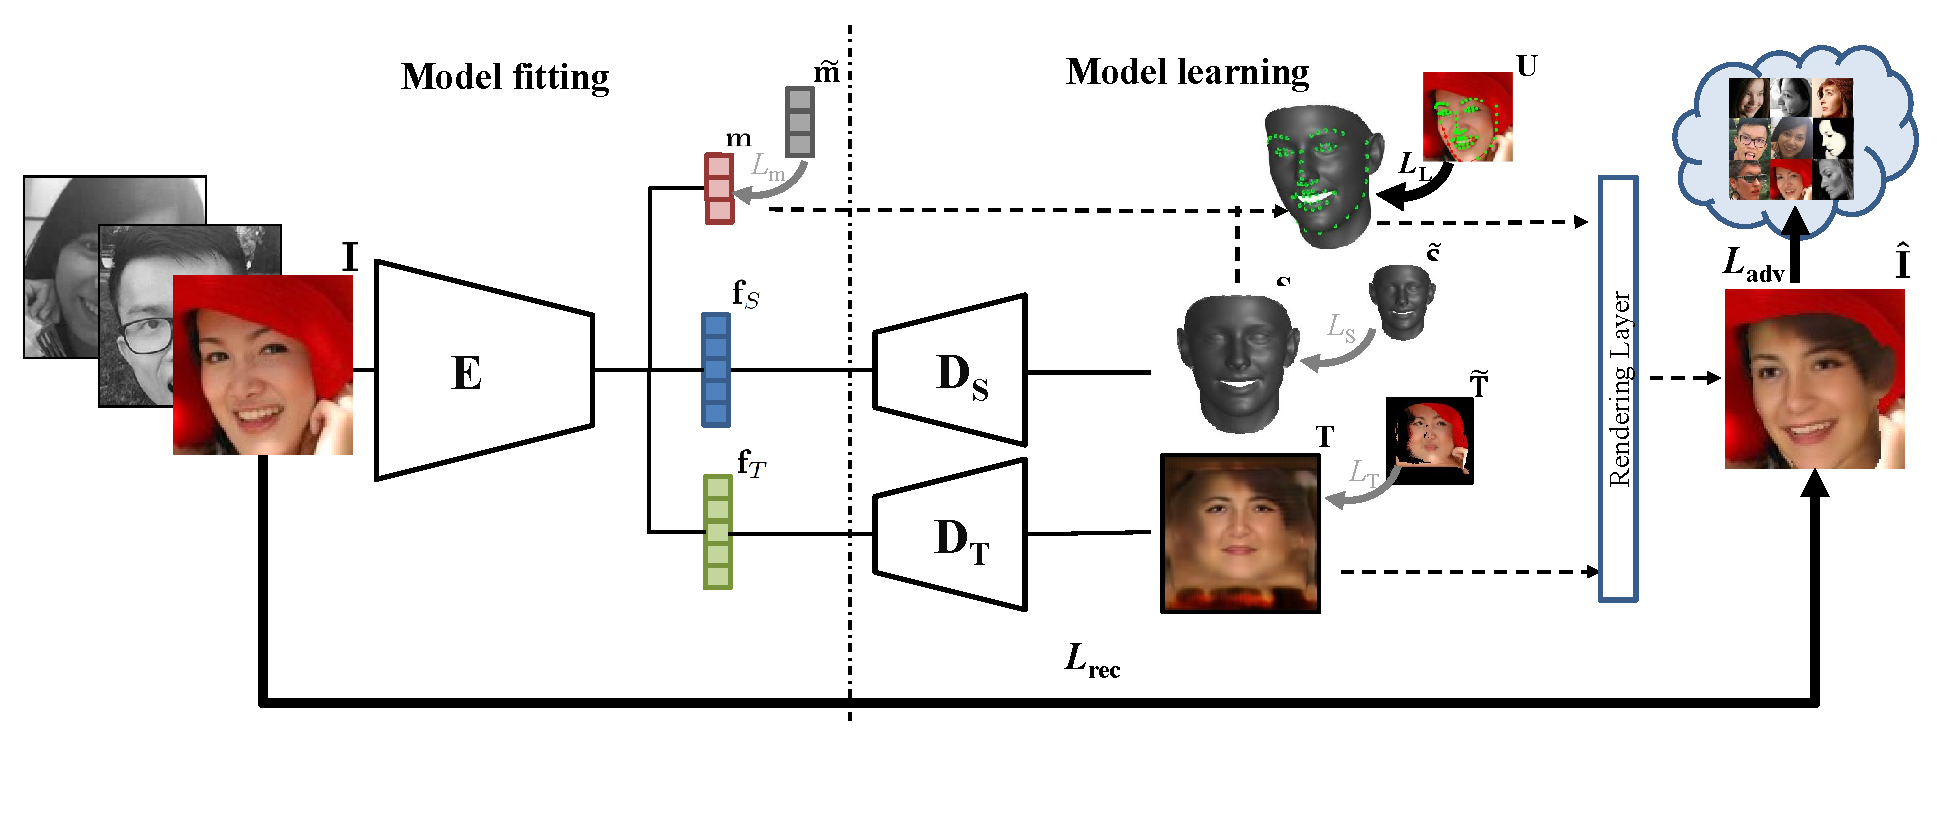
\includegraphics[trim=0 40 0 15,clip, width=0.8\linewidth]{img/Architecture.pdf}
\vspace{-3mm}
\caption{\small Jointly learning a nonlinear 3DMM and its fitting algorithm from unconstrained 2D face images, in a weakly supervised fashion.}
\label{fig:architecture}
\figvspace 
\end{figure*}


\Paragraph{3D Face Reconstruction}
3DMM also demonstrates its strength in face reconstruction. 
Since with a single image, present information about the surface is limited; 3D face reconstruction must rely on prior knowledge like 3DMM~\cite{adaptive-3d-face-reconstruction-from-unconstrained-photo-collections}. 
%Statistical PCA linear 3DMM is the most commonly used approach. 
Besides 3DMM fitting methods~\cite{blanz2003face, gu2008generative, zhang2006face,tewari2017mofa}, recently, Richardson et al.~\cite{richardson2017learning} design a refinement network that adds facial details on top of the 3DMM-based geometry.
However, this approach can only learn 2.5D depth map, which loses the correspondence property of 3DMM.
The recent work of Tewari et al.~reconstruct a 3D face by an elegant encoder-decoder network~\cite{tewari2017mofa}.
While their ability to decompose lighting with reflectance is satisfactory, our work has a different objective of learning a nonlinear 3DMM.

